% DOC SETTINGS ===================================
\documentclass{article}
\usepackage[utf8]{inputenc}
\usepackage{steinmetz}
\usepackage{mathtools}  
\usepackage{multicol}
\usepackage{circuitikz}
\usepackage{listings}
\usepackage{geometry}
\usepackage{fancyhdr}
\pagestyle{fancy}
\lhead{ECE2714 Problem Set 1}
\rhead{Kavin Thirukonda 2021}
\fancyheadoffset{0mm}
 \geometry{
 a4paper,
 total={170mm,257mm},
 left=20mm,
 top=25mm,
 }
\mathtoolsset{showonlyrefs} 
\cfoot{}
% DOC SETTINGS ===================================
\begin{document}
\begin{enumerate}
    \item Consider a signal described by the function
    \begin{equation}
        x(t) = e^{-3t}sin(10\pi t) u(t)
    \end{equation}
    \begin{enumerate}
        \item Determine the magnitude and phase of $x(\frac{1}{20})$
        \begin{align}
        x(\frac{1}{20}) & = e^{-3(\frac{1}{20})}sin(10\pi (\frac{1}{20})) u(\frac{1}{20}) \\
         & = .86sin(\frac{\pi}{2})\\
         & = .0236
        \end{align}
        \begin{center}
            Therefore the magnitude is \textbf{.0236} and the phase is \textbf{0}
        \end{center}
        \item Using Matlab, plot the signal $\lvert x(t) \lvert$ between [-2,2]. Give your code and embed the plot.
        \lstset{language=Python}
        \lstset{frame=lines}
        \lstset{label={lst:code_direct}}
        \lstset{basicstyle=\footnotesize}
        \begin{lstlisting}
        import numpy as np
        import matplotlib.pyplot as plt
        
        
        def x(t):
            return np.e ** (-3 * t) * np.sin(10 * np.pi * t) * np.heaviside(t, 0)
        
        
        t = np.linspace(-2, 2, 10000)
        plt.plot(t, abs(x(t)))
        plt.show()
        \end{lstlisting}
        \begin{center}
        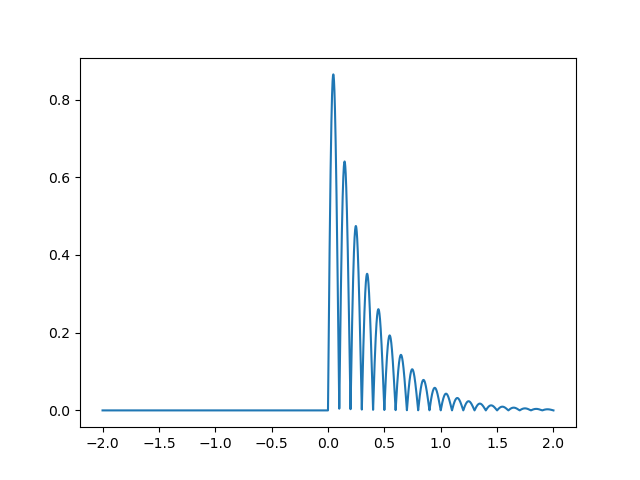
\includegraphics[width = .7\textwidth]{1b.png}    
        \end{center}
        
    \end{enumerate}
    \newpage
    \item Find a solution to the differential equation
    \begin{equation}
        \frac{dy}{dt}(t) + 9y(t) = e^{-t}
    \end{equation}
    for $t\geq0$, when $y(0) = 1$.
    \begin{center}
        Integrating Factor:
    \end{center}
    \begin{align}
        e^{\int9dt} &= e^{9t}\\
        \Rightarrow e^{9t} (y' + 9y) &= e^{9t}(e^{-t})\\
        \Rightarrow \frac{dy}{dt}(e^{9t}y)& = e^{8t}\\
        \Rightarrow e^{9t}y &= 8e^{8t} + C\\
        \Rightarrow y &= \frac{1}{8e^t} + \frac{C}{e^{9t}}
    \end{align}
    \begin{center}
        Using Initial Conditions:
    \end{center}
    \begin{equation}
        \boxed{y = \frac{1}{8e^t}+\frac{7}{8e^{9t}}}
    \end{equation}
    \itemsep 75pt
    \item Compute the integral
    \begin{equation}
        \int_{-\infty}^{\infty} e^{-t^2}\delta(t-10)dt
    \end{equation}
    where $\delta(t)$ is the delta function.
    \begin{equation}
        \int_a^bf(t)\delta(t-t_0)dt = f(t_0)
    \end{equation}
    \begin{center}
        according to the above definition:
    \end{center}
    \begin{align}
        \int_{-\infty}^{\infty} e^{-t^2}\delta(t-10)dt&= e^{-10^2}\\
        &= e^{-100}\\
        &= \boxed{3.72 * 10^{-44}}
    \end{align}
    
    \newpage
    \item Using Euler's relation $e^{j\theta} = cos\theta +jsin\theta$, show with anaytical calculations that
    \begin{equation}
        cos^2\theta = \frac{1}{2}(1+cos2\theta)
    \end{equation}
    Hint: Start by considering $e^{j(\theta +\phi)}$.
    \begin{align}
        e^{j\theta} + e^{-j\theta} &= 2cos\theta\\
        \frac{e^{j\theta} + e^{-j\theta}}{2}&=cos\theta\\
        \left(\frac{e^{j\theta} + e^{-j\theta}}{2}\right)^2&=cos^2\theta\\
        cos^2\theta &=  \left(\frac{e^{j2\theta} + 2e^{j\theta }e^{-j\theta } + e^{-j2\theta }}{4}\right)\\
        cos^2\theta &= \frac{2+2cos2\theta}{4}\\
        \end{align}
        \begin{equation}
            \boxed{cos^2\theta = \frac{1}{2}(1+cos2\theta)}    
        \end{equation}
    \item This problem concerns the finite sum formula. Show with analytical calculations that 
    \begin{equation}
        \sum_{n=0}^{N-1}\alpha^n = \begin{cases}
          N \quad & \, \alpha = 1\\
          \frac{1-\alpha^N}{1-\alpha}\quad & \,\text{for any complex number }  \alpha \ne 1 \\
     \end{cases}
    \end{equation}
    Hint: Start with the case in which $\alpha = 1$. Then consider the case in which $\alpha \ne 1$ by multiplying the term on the left-hand-side by $(1-\alpha)$.
    
    \textbf{$\alpha = 1:$}
    \begin{equation}
        \sum_{n=0}^{N-1}1^n = 1^0 + 1^1 + 1^2 + 1^3 + ... + 1^{N-1} = 1 * N = N 
    \end{equation}
    \begin{center}
        The $1^0$ term accounts for the -1 in N-1 and we end up with just N:
    \end{center}
    \begin{equation}
        \boxed{\sum_{n=0}^{N-1}1^n = N}
    \end{equation}
    \textbf{$\alpha \ne 1:$}
    \begin{align}
        (1 - \alpha) \sum_{n=0}^{N-1}\alpha^n &= \sum_{n=0}^{N-1}\alpha^n - \sum_{n=0}^{N-1}\alpha^{n+1}\\
        &= (\alpha^0 + \alpha^1 + \alpha^2 + \alpha^3 + \alpha^4 + ... + \alpha^{N-1}) - (\alpha^1 + \alpha^2 + \alpha^3 + \alpha^4 + ... + \alpha^{N-1} + \alpha^N)\\
        &= \alpha^0 - \alpha^N  = 1 - \alpha^N 
    \end{align}
    \begin{center}
        By canceling all the terms we are left with $1 - \alpha^N$ and by dividing $1 - \alpha$ back to the right side we get:
    \end{center}
    \begin{equation}
        \boxed{\sum_{n=0}^{N-1}\alpha^n  = \frac{1 - \alpha^N}{1 - \alpha}}
    \end{equation}
    \newpage
    \item Consider the complex signal
    \begin{equation}
        x(t) = e^{-3t+\frac{t}{10}j}
    \end{equation}
    \begin{enumerate}
        \item Plot $\lvert x(t) \lvert$ and \phase{x(t)}  using Matlab for $0 \leq t \leq 10$.
        \lstset{language=Python}
        \lstset{frame=lines}
        \lstset{label={lst:code_direct}}
        \lstset{basicstyle=\footnotesize}
        \begin{lstlisting}
        import numpy as np
        import matplotlib.pyplot as plt
        
        
        def x(t):
            return np.e**(-3*t+t*.1j)
        
        
        t = np.linspace(0, 10, 10000)
        plt.plot(t, abs(x(t)))
        plt.title("Magnitude")
        plt.show()
        plt.plot(t, np.angle(x(t)))
        plt.title("Phase")
        plt.show()
        \end{lstlisting}
        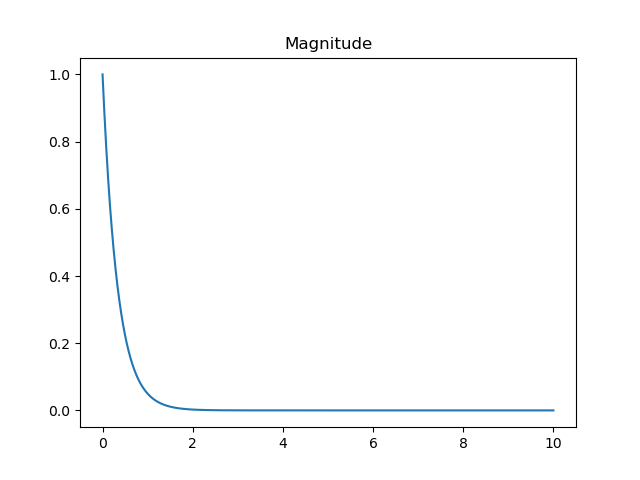
\includegraphics[width = .7\textwidth]{6aM.png}
        
        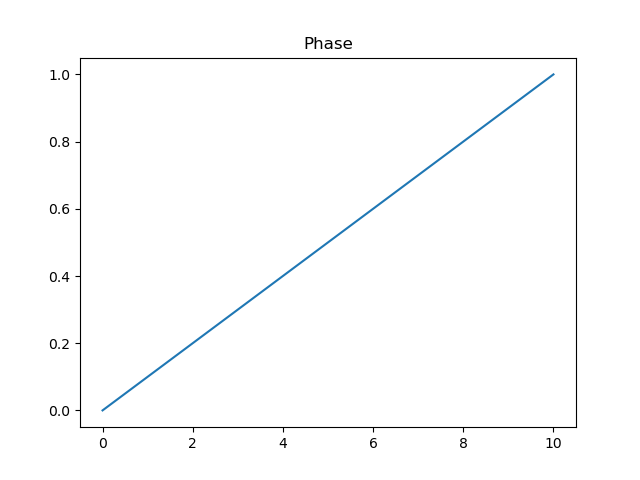
\includegraphics[width = .7\textwidth]{6aP.png}
        \item Determine y(t) if
        \begin{align}
            y(t) &= \int  x(t)dt\\
            &= \int e^{-3t+\frac{t}{10}j}dt\quad u = -3t + \frac{t}{10}j\\
            &= \int \frac{10e^u}{-30+j}du\\
            &= \frac{10}{-30+j}\cdot \int e^udu\\
            &= \boxed{\frac{10}{-30+j}\cdot e^{-3t + \frac{t}{10}j} + C}
        \end{align}
        \item Determine W if 
        \begin{align}
            W &= \int_0^{10} x(t)dt\\
            &= \frac{10}{-30+j}\cdot e^{-3t + \frac{t}{10}j}\bigg]_0^{10}\\
            &= \frac{10}{-30+j}\cdot e^{-3(10) + \frac{(10)}{10}j}-1\\
            &= \boxed{-\frac{4}{3}-j \cdot e^{-30+j}}
        \end{align}
        \item Determine y(t) if
        \begin{align}
            y(t) &= \int_0^t x(t)dt\\
            &= \frac{10}{-30+j}\cdot e^{-3t + \frac{t}{10}j}\bigg]_0^{t}\\
            &= \frac{10}{-30+j}\cdot e^{-3(t) + \frac{(10)}{t}j}-1\\
            &= \boxed{-\frac{4}{3}-j \cdot e^{-3t+j}}
        \end{align}
    \end{enumerate}
   
    \newpage
    \item Consider a signal represented by the function x(t) where
    \begin{equation}
        x(t) = cos(2t)u(t)
    \end{equation}  
    \lstset{language=Python}
    \lstset{frame=lines}
    \lstset{label={lst:code_direct}}
    \lstset{basicstyle=\footnotesize}
    \begin{lstlisting}
    import numpy as np
    import matplotlib.pyplot as plt
    
    
    def x(t):
        return np.cos(2*t)*np.heaviside(t, 0)
    
    
    t = np.linspace(-1, 3, 10000)
    plt.plot(t, x(t))
    plt.show()
    plt.plot(t, x(2*t))
    plt.show()
    plt.plot(t, x(t+2))
    plt.show()
    \end{lstlisting}
    \begin{multicols*}{2}
    \begin{enumerate}
        \item Plot x(t) for $-1 \leq t \leq 3$
        
        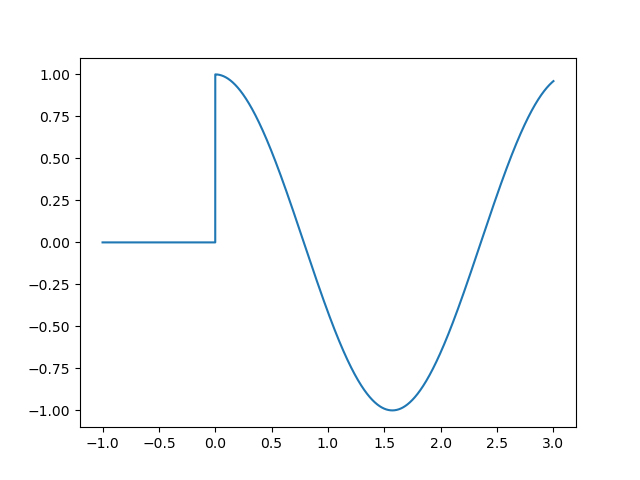
\includegraphics[width = .41\textwidth]{7a.png}
        \item Plot x(2t) for $-1 \leq t \leq 3$
        
        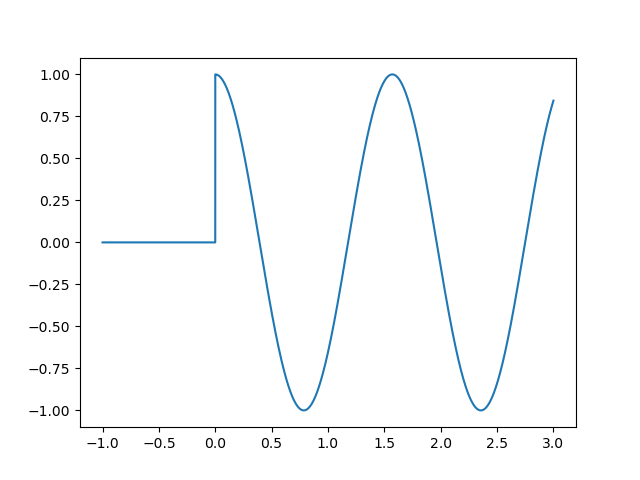
\includegraphics[width = .41\textwidth]{7b.png}
        \item Plot x(t+2) for $-1 \leq t \leq 3$
        
        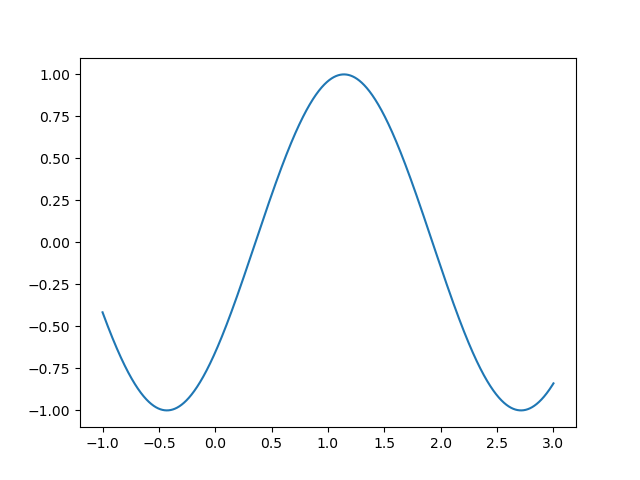
\includegraphics[width = .41\textwidth]{7c.png}
        \item Is x(t) an even or odd function?
        \begin{center}
            \textbf{Neither}, because there is a step function included which makes the function invalid for both even and odd.
        \end{center}
        \itemsep 115pt
        \item is x(t) periodic?
        \begin{center}
            \textbf{No}, because there is a step function so it is not true for the entire number line.
        \end{center}
        \itemsep 125pt
        \item Is x(t) a power signal (one with finite power but infinite energy), an energy signal (one with finite energy but zero power), or neither?
        \begin{center}
            The signal x(t) is a \textbf{power signal} and therefore has finite power and infinite  energy. This can be concluded by plugging the function into the power integral, or by examining the graph logically.
        \end{center}
    \end{enumerate}
    \end{multicols*}
\end{enumerate}

\end{document}
